% -*- latex -*-
%%%%%%%%%%%%%%%%%%%%%%%%%%%%%%%%%%%%%%%%%%%%%%%%%%%%%%%%%%%%%%%%
%%%%%%%%%%%%%%%%%%%%%%%%%%%%%%%%%%%%%%%%%%%%%%%%%%%%%%%%%%%%%%%%
%%%%
%%%% This text file is part of the source of 
%%%% 'Parallel techniques'
%%%% by Ángel de Vicente, copyright 2019
%%%%
%%%% TO DO:
%%%%  + Add stuff as text, not as images from the manuals
%%%%  + Add a visual description of the N-body problem
%%%%     (animation, video?)
%%%%
%%%% nbody.tex : basic N-body problem formulation
%%%%
%%%%%%%%%%%%%%%%%%%%%%%%%%%%%%%%%%%%%%%%%%%%%%%%%%%%%%%%%%%%%%%%
%%%%%%%%%%%%%%%%%%%%%%%%%%%%%%%%%%%%%%%%%%%%%%%%%%%%%%%%%%%%%%%%

\Level 0 {Introduction}
\label{sec:naive-nbody}

A nice introduction to the N-Body problem can be found in the documentation for
the XStar\footnote{http://www.schlitt.net/xstar/} code: ``The ``N-Body problem''
is the problem of trying to find how n objects will move under one of the
physical forces, such as gravity.'' \cite{Schlitt_2000}. The XStar code (written
in the C language) solves what we will cover in this course and more, except for
the parallelization part. Figure \ref{fig:xstar1} shows an example screenshot of
a simulation run with XStar.

\begin{figure}[!htbp]
  \centering
  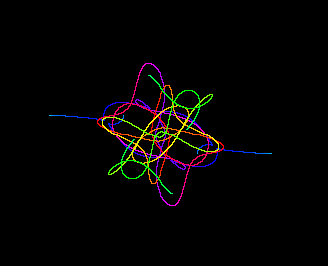
\includegraphics[width=0.5\textwidth]{graphics/xstar1.png}
  \label{fig:xstar1}
  \caption{Sample XStar configuration simulation (from http://www.schlitt.net/xstar/screen\_shots.html)}
\end{figure}


\Level 0 {N-body equations}
\label{sec:nbody-equation}


The equations to solve the N-body problem are very simple. See, for example,
sections 1.2 and 1.3 of the Xstar guide
(http://www.schlitt.net/xstar/n-body/nb-8.html), and page 65 of ``Moving Stars
Around''.

\begin{figure}[!htbp]
  \centering
  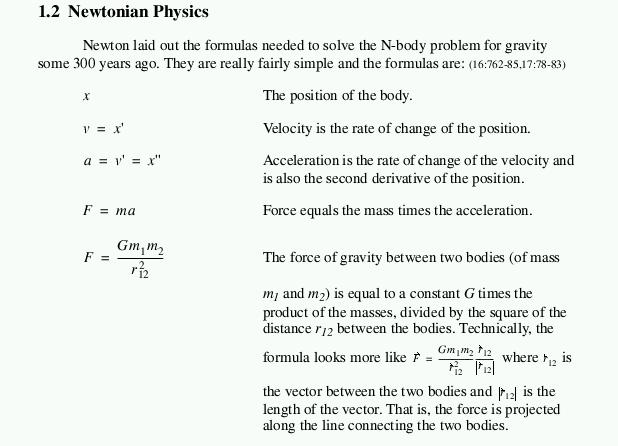
\includegraphics[width=\textwidth]{graphics/nbody-fig1.png}
  \caption{p.8 Guía Xstar}
\end{figure}


\begin{figure}[!htbp]
  \centering
  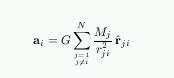
\includegraphics[width=0.3\textwidth]{graphics/nbody-fig2.png}
  \caption{p. 65 ``Moving Stars Around''}
\end{figure}

\Level 0 {Time integration}
\label{sec:nbody-time-integration}


To integrate in time, one can use several methods. The simplest one, of order 1
is Forward-Euler, as can be seen in page 24 of ``Moving Stars
Around''. The one we are going to use here is of order 2: the leapfrom algorithm
(see pages 55-56 of ``Moving Stars Around'').

\begin{figure}[!htbp]
  \centering
  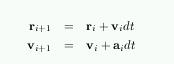
\includegraphics[width=0.3\textwidth]{graphics/nbody-fig3.png}
  \caption{p.24 ``Moving Stars Around''}
\end{figure}

\begin{figure}[!htbp]
  \centering
  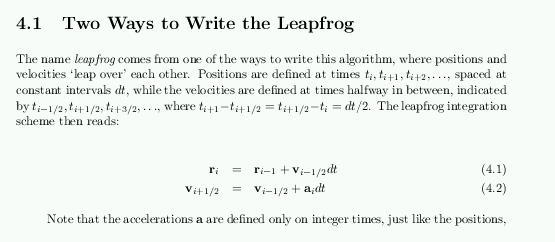
\includegraphics[width=\textwidth]{graphics/nbody-fig4.png}
  \caption{p.55 ``Moving Stars Around''}
\end{figure}

\begin{figure}[!htbp]
  \centering
  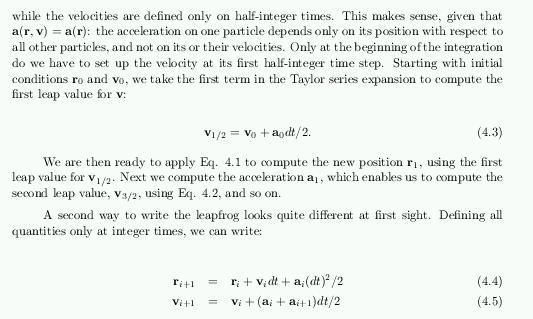
\includegraphics[width=\textwidth]{graphics/nbody-fig5.png}
  \caption{p.56 ``Moving Stars Around''}
\end{figure}

